\documentclass[UTF8]{ctexart}
\usepackage{geometry}
\geometry{left=2.5cm,right=2.5cm,top=2.5cm,bottom=2.5cm}
\usepackage[raggedright]{titlesec}
\usepackage{enumerate}
\usepackage{amsmath}
\usepackage{amssymb}
\usepackage[colorlinks, linkcolor = blue]{hyperref}
\usepackage[nameinlink, capitalize]{cleveref}
\usepackage{cite}
\usepackage{tikz}
\usepackage{float}
\allowdisplaybreaks[4]

\title{题目待定}

\begin{document}
\maketitle
\section{课题背景及研究意义}
\label{background}
本文的研究来源于云制造二期项目关于“集团企业云制造平台关键技术研究应用”的相关研究要求。该项目主要研究内容包括集团企业应用模式研究,资源服务组合优化调度及集团企业云制造服务平台研发等。云制造作为一种网络化制造的新模式,其概念、构成、关键技术、运营模式等都已得到了广泛的研究。根据课题及实际生产制造的需求,本文选取云制造环境作为研究背景,从云制造大环境下单个企业的视角出发,旨在研究单个企业的自主决策以及资源服务优化调度问题。

资源服务组合优化问题作为云制造二期项目的其中一个主要研究内容,有其重要的研究意义和复杂性。这里就其研究意义进行具体阐述:
\begin{enumerate}[(i)]
\item 在云制造运营模式下,资源服务与需求之间本质上是多对多的关系,平台匹配与优化组合的结果通常直接为企业提供决策支持;而企业的决策调度结果反过来又会影响到平台运营,进而影响到整个云制造系统的运作效率。
\item 云制造从其提出至今已逾六年,关于其概念和意义的研究基本已有定论。而其运营模式的讨论和关键技术的研究目前仍在继续。云制造资源服务组合优化问题作为支撑云制造的其中一项关键技术,将不可避免地成为下一轮研究的重点。
\item 大系统的组合优化问题通常是具有$\mathcal{NP}$难度的。$\mathcal{NP}$类问题由于其理论意义与求解的困难程度广泛地被各个领域的学者所关注。云制造资源服务组合优化问题作为这类问题的一个典型代表不但能引起研究者的研究兴趣,而且也兼具实际应用价值。
\end{enumerate}
% 由于云制造平台上往往聚集着海量的制造资源和服务,资源服务与用户需求之间的匹配和组合优化的有效性直接影响到企业决策,进而影响到平台运营。

\section{国内外研究现状}
\label{present research situation}
云制造这个概念最早由李伯虎团队\cite{LiBohu2010}于2010年提出。在其论文中,李伯虎团队首先提出了“分散资源集中使用,集中资源分散服务”的云制造思想,并将云制造与应用服务提供商和制造网格进行区分。此外,他们还分析了云制造的体系结构及实现云制造所需的关键技术。

Xu\cite{Xu2012}通过分析云计算的特征,认为云计算将会与传统的制造业相结合从而形成新的企业运营模式。Xu还认为云计算与制造主要有直接将云计算应用于制造系统和云制造这两种结合方式,并列举了一些目前在制造业中已经出现的应用云计算的运营模式的案例。

Tao等\cite{Tao2011}讨论了云制造的概念、构成和典型特征,提出了四种类型的云制造服务平台,并总结了云计算和云制造的关系。

Zhang等\cite{Zhang2014}将云制造视为一种结合了云计算技术、物联网技术和面向服务技术的一种新的制造范式。通过研究其构成、典型特征以及关键技术,他们认为云制造主要由以下三部分组成:云制造资源、制造云服务和制造云。

Tao等\cite{Tao2014}修改并建立了云服务中的计算资源最优化分配(Optimal Scheduling of Computing Resources, OSCR)问题模型,以完工时间和能耗为优化目标,采用混合遗传算法进行求解。

Laili等\cite{Laili2012}针对云制造中计算资源最优化分配(Optimal Allocation of Computing
Resources, OACR)问题,提出了一种新的利基免疫算法(Niche Immune Algorithm),并对该问题进行求解。

Lartigau等\cite{6227791}尝试对云制造中的订单任务进行调度。

针对基于企业系统的云制造资源组合优化问题,Tao等\cite{6376181}提出了一种新的并行智能算法并对该问题进行求解。

以云制造环境下单个企业的视角来看,企业面临自主决策是否接受订单并对其进行调度的问题。这类问题被称为订单接受及其调度(Order Acceptance and Scheduling, OAS)问题。Oguz等\cite{Og2010}研究了单机环境下的OAS问题并用启发式算法得到了较为满意的解。

针对单机的OAS问题,Nguyen等\cite{Nguyen2015}采用了基于遗传算法的分派规则进行求解,并取得了一定的效果。

Wang等\cite{Wang2013}研究了两台机器的流水车间环境下的OAS问题,结合分支定界和启发式算法,对于大量随机实例,他们给出了优于CPLEX的求解算法及结果。

在网络化制造大环境下,在制造过程中企业间必然存在着相互协同。Qi\cite{Qi2011}研究了两阶段流水线的制造外包问题,提出了三种外包的形式,并用动态规划进行了求解。

% 在云制造环境下,资源服务的需求方同时也可以是资源服务的提供方。

\section{研究内容及问题建模}
\label{model}
在不同的云制造平台运营模式下,云制造加盟企业的组织形式不会完全相同。因此,在研究云制造中的资源服务组合优化问题之前,首先要讨论云制造的运营模式。如果不确定云制造平台的运营模式,资源服务组合优化问题将无从谈起。

\subsection{云制造平台运营模式}
\label{forms of platform}
基于一些前期的讨论和参考目前现有的一些商业运作模式,我们认为云制造平台的运营模式不外乎以下三种:平台强控制模式,平台弱控制模式,以及介于两者之间的平台推荐模式。

\begin{enumerate}[(i)]
\item \textbf{平台强控制模式}:平台强控制模式类似于无人化工厂,云制造的每个加盟企业都可视为一个分布式车间,加盟企业提供制造资源,统一由云平台调控。对于共享的制造资源,在其受云平台调控期间,加盟企业无权对其进行调控。当服务需求方提出制造要求时,由平台进行统一的制造安排并实施生产制造。这种模式的优势在于,云平台由于掌握着整个制造系统的所有信息,因此往往能给出较优的总体利益最大化的调度方案;其劣势也很明显,比如利益分配困难、总体调度难以找到满意解、实施困难等等。
\item \textbf{平台弱控制模式}:在平台弱控制模式中,平台可以视为一个容器。在这个容器中有海量的需求和服务,用户自行搜索所需的服务,平台作为中介方实施管理。这种模式的优势在于其实施非常方便,管理也很容易;但是其劣势在于,缺乏了平台对资源服务的制导,服务需求方难以找到满意的服务,整个系统运作效率较低。
\item \textbf{平台推荐模式}:平台推荐模式介于以上两种模式之间。平台方接受服务需求方提交的订单,为其匹配最合适的资源服务提供企业。服务的提供企业有权力选择是否接受该订单。如果该企业不愿接受该订单,云平台会为该订单寻找次优的企业,直到有企业愿意接受,才开始安排生产制造。如果没有企业愿意接受该项订单,该项订单将退回订单提交方。这种模式的优点在于,较于平台强控制模式,其实施和管理简单很多,而且也充分考虑了服务提供企业的意愿;其缺点在于,由于平台只对服务提供企业进行推荐而并不安排生产制造,服务提供企业面临复杂的决策问题,其最终的决策结果也会影响到整个制造系统的运作效率。

\end{enumerate}

综合考虑这三种模式的优缺点,本文选取平台推荐模式作为课题研究的背景。

\subsection{云制造环境下企业的订单选择和调度模型}
\label{concrete model}
在采用推荐模式的云平台上运作的制造系统中,资源服务的提供企业需要对到达的订单进行决策调度,从而最大化企业资源的效益。

为便于说明云制造环境下企业的订单选择和调度模型,这里以单机问题为例进行阐述。假设某企业目前只有一台机器设备,一个订单就是一个不可再分的任务,一台机器上同一个时刻只能加工一个任务,且这些任务是不可中断的。不妨假设当前时刻为$\mu_0 T$时刻且恰好为资源服务提供企业的决策调度时刻,企业的决策调度间隔时间为$T$。$S^t$表示企业在$t$时刻的调度状态,比如$S^{\mu_0 T}$表示当前时刻企业的调度状态,$S^{(\mu_0 - 1)T}$表示在时刻$(\mu_0 - 1)T$(也就是上一次调度的时刻)企业的调度状态,$S^{(\mu_0 + 1)T}$表示在时刻$(\mu_0 + 1)T$(也就是下一次调度的时刻)企业的调度状态。在每个调度时刻,企业根据平台推荐的在该时刻的可选订单集$\Omega^t$和该时刻企业的调度状态$S^t$,决定接受哪些订单并对其进行调度。由于在这种云平台模式下,一项订单可能会被多个企业拒绝后才被下一个企业接受,因此每项订单$O_j$对应不同企业$E_l$具有不同的订单决策开始时间$ds_{jl}$和订单决策结束时间$de_{jl}$。在每个调度时刻,企业接受但未开始生产制造的订单集记为$\Phi^t$。订单$O_j$的释放时间和工期分别记为$r_j$和$d_j$,收益是与完工时间有关的函数$e_j(t)$。每项企业接受但还未释放的订单均可外包且外包件都可在工期内完成,外包成本为$l_j$(通常情况下$l_j > e_j(r_j)$)。在每个调度时刻$\mu T$($\mu$ 为整数),企业需要将上一次调度状态$S^{(\mu - 1)T}$更新为$S^{\mu T}$,使得其在$\mu T$时刻企业的调度收益最大。

\begin{figure}[H]
\centering
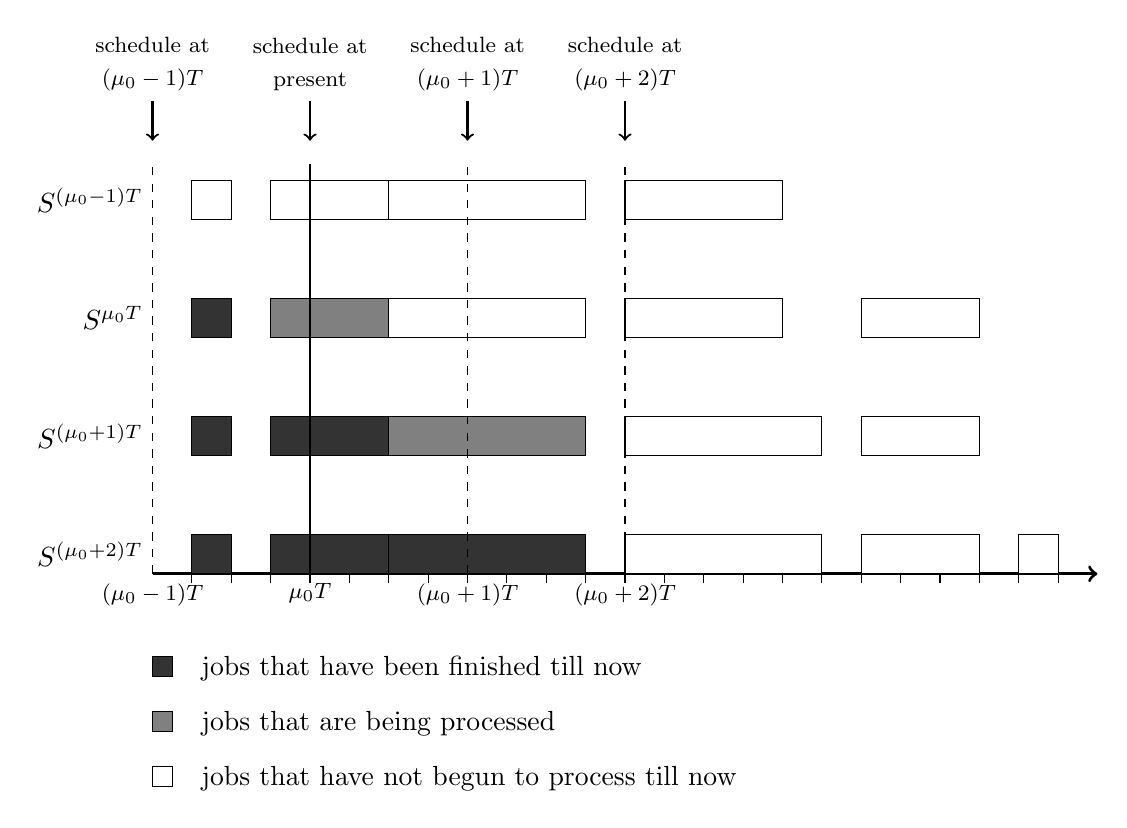
\begin{tikzpicture}[scale = 1]
	\draw [->] [very thick] (-2, 0) -- (10, 0);
	\foreach \x in {-1.5, -1, ..., 9.5}
		\draw (\x, -3.5pt) -- (\x, 3.5pt);

	\filldraw [fill = white] (-1.5, 4.5) rectangle +(0.5, 0.5);
	\filldraw [fill = white] (-0.5, 4.5) rectangle +(1.5, 0.5);
	\filldraw [fill = white] (1, 4.5) rectangle +(2.5, 0.5);
	\filldraw [fill = white] (4, 4.5) rectangle +(2, 0.5);

	\filldraw [fill = white!20!black] (-1.5, 3) rectangle +(0.5, 0.5);
	\filldraw [fill = gray] (-0.5, 3) rectangle +(1.5, 0.5);
	\filldraw [fill = white] (1, 3) rectangle +(2.5, 0.5);
	\filldraw [fill = white] (4, 3) rectangle +(2, 0.5);
	\filldraw [fill = white] (7, 3) rectangle +(1.5, 0.5);

	\filldraw [fill = white!20!black] (-1.5, 1.5) rectangle +(0.5, 0.5);
	\filldraw [fill = white!20!black] (-0.5, 1.5) rectangle +(1.5, 0.5);
	\filldraw [fill = gray] (1, 1.5) rectangle +(2.5, 0.5);
	\filldraw [fill = white] (4, 1.5) rectangle +(2.5, 0.5);
	\filldraw [fill = white] (7, 1.5) rectangle +(1.5, 0.5);

	\filldraw [fill = white!20!black] (-1.5, 0) rectangle +(0.5, 0.5);
	\filldraw [fill = white!20!black] (-0.5, 0) rectangle +(1.5, 0.5);
	\filldraw [fill = white!20!black] (1, 0) rectangle +(2.5, 0.5);
	\filldraw [fill = white] (4, 0) rectangle +(2.5, 0.5);
	\filldraw [fill = white] (7, 0) rectangle +(1.5, 0.5);
	\filldraw [fill = white] (9, 0) rectangle +(0.5, 0.5);

	\draw [dashed] (-2, 0) -- (-2, 5.2);
	\draw (0, 0) -- (0, 5.2);
	\draw [dashed] (2, 0) -- (2, 5.2);
	\draw [dashed] (4, 0) -- (4, 5.2);
	\draw [->] [thick] (-2, 6) node [anchor = south, align=center] {\footnotesize schedule at \\ \footnotesize $(\mu_0 - 1)T$} -- (-2, 5.5);
	\draw [->] [thick] (0, 6) node [anchor = south, align=center] {\footnotesize schedule at \\ \footnotesize present} -- (0, 5.5);
	\draw [->] [thick] (2, 6) node [anchor = south, align=center] {\footnotesize schedule at \\ \footnotesize $(\mu_0 + 1)T$} -- (2, 5.5);
	\draw [->] [thick] (4, 6) node [anchor = south, align=center] {\footnotesize schedule at \\ \footnotesize $(\mu_0 + 2)T$} -- (4, 5.5);

	\draw (0, 0) node [anchor = north] {\footnotesize $\mu_0 T$};
	\draw (-2, 0) node [anchor = north] {\footnotesize $(\mu_0 - 1)T$};
	\draw (2, 0) node [anchor = north] {\footnotesize $(\mu_0 + 1)T$};
	\draw (4, 0) node [anchor = north] {\footnotesize $(\mu_0 + 2)T$};

	\draw (-2, 4.75) node [anchor = east] {$S^{(\mu_0 - 1)T}$};
	\draw (-2, 3.25) node [anchor = east] {$S^{\mu_0 T}$};
	\draw (-2, 1.75) node [anchor = east] {$S^{(\mu_0 + 1)T}$};
	\draw (-2, 0.25) node [anchor = east] {$S^{(\mu_0 + 2)T}$};

	\filldraw [fill = white!20!black] (-2, -1.3) rectangle +(0.25, 0.25);
	\draw (-1.5, -1.2) node [anchor = west] {jobs that have been finished till now};
	\filldraw [fill = gray] (-2, -2) rectangle +(0.25, 0.25);
	\draw (-1.5, -1.9) node [anchor = west] {jobs that are being processed};
	\filldraw [fill = white] (-2, -2.7) rectangle +(0.25, 0.25);
	\draw (-1.5, -2.6) node [anchor = west] {jobs that have not begun to process till now};

\end{tikzpicture}
\caption{云制造环境下企业的订单选择和调度模型的一个实例}
\label{Fig: IllofOASwithTimeHorizon}
\end{figure}

这类问题有点类似于基于接受拒绝的调度(Interval Scheduling, IS)模型\cite{Bouzina, Kolen2007}。\cref{Fig: IllofOASwithTimeHorizon}给出了云制造环境下企业的订单选择和调度模型的一个实例。在调度时刻$(\mu_0 - 1)T$,企业接受了四个订单并调度好了生产制造的时段,此时的企业调度状态为$S^{(\mu_0 - 1)T}$。在调度时刻$\mu_0 T$,也即为当前调度时刻,先前的四个订单中有一个已经完成,一个正在加工,另外两个还未开始加工。此外,由于在时间段$((\mu_0 - 1)T,\ \mu_0 T]$内有新的订单到达,此时的企业调度状态为$S^{\mu_0 T}$。在下一个调度时刻$(\mu_0 + 1)T$(当前时刻并不知道下个调度时刻会发生什么,假设那时企业的调度状态就如图所示),两个订单已经完成,一个订单正在加工。上个时刻安排加工的一个订单,由于在时间段$(\mu_0 T,\ (\mu_0 + 1)T]$内将到达一个更具有价值的订单,企业选择将其外包而自己加工更有价值的订单。此时企业的调度状态将为$S^{(\mu_0 + 1)T}$。同理,在调度时刻$(\mu_0 + 2)T$,企业的调度状态将为$S^{(\mu_0 + 2)T}$。最后,在时间轴上深色部分的订单即为企业最后真正加工的订单(企业外包的订单在这里没有显示)。

\subsection{单机问题的数学模型}
\label{math model}
在每个调度时刻$\mu T$($\mu = 0,\ 1,\ 2,\ \dots$),企业都面临着一个决策优化问题,而当订单的收益$e_j(t)$随时间是分段线性时,该问题实际上是一个混合整数线性规划问题(Mixed Iteger Linear Programming, MILP)。为了说明问题,简单起见,这里认为$e_j(t)$如\cref{eq: e_j(t) value}取值,其中$C_j$为订单$O_j$的制造期。令$I_j$为决策变量,$I_j$决策企业是否接受并加工制造订单$O_j$,其取值如\cref{eq: I_j}所示。令$y_{jk}$为决策变量,用来对企业接受的订单进行排序,其取值如\cref{eq: y_jk}所示。记订单$O_j$的延迟为$T_j$,收益为$R_j$,加工时间为$p_j$。令$m$为集合$\Omega^{\mu T}$的元素个数,$n$为集合$\Phi^{\mu T}$的元素个数,$t_0$为$\mu T$之后最早可开始调度时间。
\begin{flalign}\label{eq: e_j(t) value}
& e_j(t) = \begin{cases}
e_j, & \text{if}\ C_j \leqslant d_j; \\
e_j - \omega_j (C_j - d_j), & \text{otherwise}.
\end{cases} &
\end{flalign}

\begin{flalign}\label{eq: I_j}
& I_j = \begin{cases}
1, & \text{oder $j$ is accepted and planned to process by enterprise}; \\
0, & \text{otherwise}.
\end{cases} &
\end{flalign}

\begin{flalign}\label{eq: y_jk}
& y_{jk} = \begin{cases}
1, & \text{if order $j$ precedes order $k$, \quad $i,j \in (\Omega^{\mu T} \cup \Phi^{\mu T})$}; \\
0, & \text{otherwise}.
\end{cases} &
\end{flalign}

该MILP问题为:

\begin{flalign}
& \text{Maximize} \sum\limits_{j = 1}^{m + n} R_j &\quad& &\quad& \notag \\[0.35cm]
& \text{s.t.} & & & &\notag \\[0.35cm]
& \sum\limits_{k = 1,\ k \ne j}^{m + n + 1} y_{jk} = I_j & & \forall j = 0, \dots, m + n & & \label{eq: precedes only one order} \\[0.35cm]
& \sum\limits_{k = 0,\ k \ne j}^{m + n} y_{kj} = I_j & & \forall j = 1, \dots, m + n + 1 & & \label{eq: succeeded only one order} \\[0.35cm]
& C_j y_{jk} + p_k y_{jk} \leqslant C_k & & \forall j = 0, \dots, m + n,\ \forall k = 1, \dots, m + n + 1,\ j \ne k & & \label{eq: sequence} \\[0.35cm]
& (r_j + p_j)I_j \leqslant C_j & & \forall j = 0, \dots, m + n + 1 & & \label{eq: process time constraint 1} \\[0.35cm]
& (t_0 - \mu T + p_j)I_j \leqslant C_j & & \forall j = 0, \dots, m + n + 1 & & \label{eq: process time constraint 2} \\[0.35cm]
& T_j \geqslant 0 & & \forall j = 0, \dots, m + n + 1 & & \label{eq: start time 1} \\[0.35cm]
& T_j \geqslant C_j - d_j & & \forall j = 0, \dots, m + n + 1 & & \label{eq: start time 2} \\[0.35cm]
& R_j \leqslant e_j I_j - T_j \omega_j & & \forall j = 1, \dots, m & & \label{eq: revenue 1} \\[0.35cm]
& R_j \leqslant e_j - l_j(1 - I_j) - T_j \omega_j & & \forall j = m + 1, \dots, m + n & & \label{eq: revenue 2} \\[0.35cm]
& C_0 = t_0 - \mu T, \ C_{m + n + 1} = \max \limits_{j = 1, \dots, m + n} \{ C_j \} & & & & \label{eq: C} \\[0.35cm]
& I_0 = 1, I_{m + n + 1} = 1 & & & & \label{eq: I} \\[0.35cm]
& I_j \in \{0, 1\},\ y_{jk} \in \{0, 1\} & & \forall j = 0, \dots, m + n,\ \forall k = 1, \dots, m + n + 1, j \ne k & & \label{eq: I y}
\end{flalign}

\cref{eq: precedes only one order}和\cref{eq: succeeded only one order}保证了如果订单$j$被接受,它至多只有一道紧后或者紧前工序。\cref{eq: sequence}表示如果订单$k$在订单$j$后开始加工,订单$k$的制造期所满足的约束;如果订单$k$不在$j$后加工,只需满足$C_j \geqslant 0$。\cref{eq: process time constraint 1}和\cref{eq: process time constraint 2}表示订单$j$的释放时间、加工时间和制造期之间的关系。\cref{eq: start time 1}和\cref{eq: start time 2}表示订单延迟。\cref{eq: revenue 1}表示当前调度新接受的订单的收益,\cref{eq: revenue 2}表示上一次调度接受但到当前调度还未开始加工的订单的收益(其中包括外包成本)。\cref{eq: C}为虚拟制造期$C_0$和$C_{m + n + 1}$的取值。\cref{eq: I}为$I_0$和$I_{m + n + 1}$的取值。\cref{eq: I y}表示决策变量$I_j$和$y_{jk}$均为$0-1$变量。


\section{拟采用的求解方法}
\label{solution}
在\cref{model}中,以单机模型为例,简略地介绍了一下推荐模式的云制造环境下企业的订单决策和调度问题。在实际生产制造中,机器环境远比单机环境要复杂得多。在机器环境比较简单时(比如单机环境),这类问题用MILP形式表述比较清晰;当机器环境比较复杂时,用约束规划(Constraint Programming, CP)的形式表述更恰当。对于MILP形式表述的问题模型,一般常用分支定界法(Branch and Bround, B\&B)结合一些启发式算法对该问题的上界(Upper Bound, UB)和下界(Lower Bound, LB)进行压缩,最终获得满意解。对于用CP形式表述的问题模型,由于其问题比较复杂,一般用一些元启发式算法结合邻域搜索求解比较方便。

除了\cref{math model}中对于某个调度时刻而言的优化调度问题外,调度周期$T$的确定也是至关重要的,$T$可能可以作为另一个优化问题的决策变量来考虑。除此之外,\cref{model}中并未对介于两个调度时刻内需要决策的订单进行考虑,比如$[ds_{jl},\ de_{jl}] \subset ((\mu - 1)T,\ \mu T)$的情况。这类订单应当设计一些其它的规则进行决策。


\bibliographystyle{unsrt} 
\bibliography{D:/biblib/science.bib} 
\end{document}